\begin{frame}{Support Vector Machine (SVM)}
    \begin{itemize}
        \item Extends the support vector classifier by using \textbf{kernel functions} to achieve non-linear decision boundaries.
    \end{itemize}

    \centering
    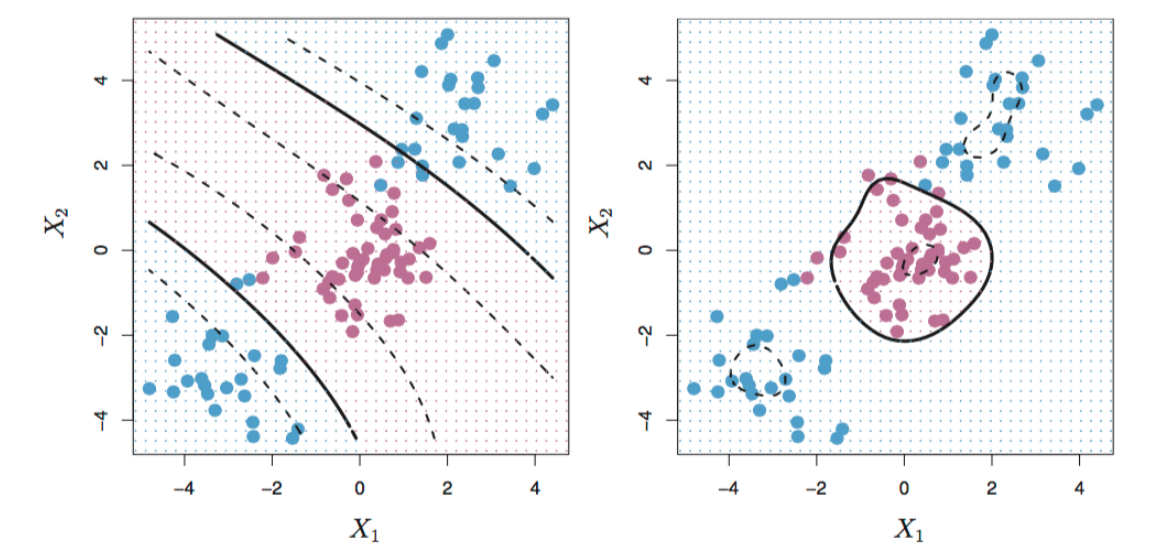
\includegraphics[width=0.9\textwidth]{images/support-vector-machines/support-vector-machines-21.png}
\end{frame}


\begin{frame}{Support Vector Machine (SVM)}
    \begin{itemize}
        \item \textbf{Kernel function:} generalization of inner product. It takes in two arguments and \textit{implicitly} computes their inner product in some feature space.
        \item Kernels are an efficient computational approach to create non-linear decision boundaries.
        \item They (implicitly) map data into a higher-dimensional space.
        \item We then apply a support vector classifier in this high-dimensional space with a linear decision boundary (hyperplane).
    \end{itemize}
\end{frame}


\begin{frame}{Linear SVM}
    It can be shown that a support vector classifier can be represented as:

    \[
    f(x) = \beta_0 + \sum_{i \in S} \alpha_i \langle x, x_i \rangle
    \]

    
    \begin{itemize}
        \item $f(x) > 0$ is one class, $f(x) < 0$ is another
        \item $S$ is the set of support vectors
        \item $\langle x, x_i \rangle$ is the \textbf{inner product}
    \end{itemize}
    
    \textbf{Where:}
    \[
    \langle \vec{u}, \vec{v} \rangle = \sum_{j=1}^{p} u_j v_j
    \]
\end{frame}


\begin{frame}{General SVM}
    It can be shown that a support vector classifier can be represented as:

    \[
    f(x) = \beta_0 + \sum_{i \in S} \alpha_i \langle x, x_i \rangle
    \]

    \vspace{0.6cm}

    In SVM, we replace the inner product with a kernel function:

    \[
    f(x) = \beta_0 + \sum_{i \in S} \alpha_i K\left(x^{(i)}, x\right)
    \]
\end{frame}

\begin{frame}{Properties of Kernels}
    \begin{itemize}
        \item \textbf{Generalization of inner product:}
        \[
        \text{for an explicit feature map} \quad \phi : \mathcal{X} \rightarrow \mathcal{X}^\phi, \quad x \mapsto \phi(x)
        \]
        \[
        K(x, x') = \langle \phi(x), \phi(x') \rangle_{\mathcal{X}^\phi}
        \]

        \item \textbf{Symmetric:} \quad $K(x, x') = K(x', x)$

        \item \textbf{Gives a measure of similarity} between $X$ and $X'$
        \begin{itemize}
            \item If $X$ and $X'$ are close together, then $K(X, X')$ is large
            \item If $X$ and $X'$ are far apart, then $K(X, X')$ is small
        \end{itemize}
    \end{itemize}

    {\tiny For a more formal definition: \url{http://mlweb.loria.fr/book/en/constructingkernels.html}}
\end{frame}


\begin{frame}{Common SVM Kernels}
    \begin{itemize}
        \item \textbf{Linear kernel}
        \[
        K(x, x') = \langle x, x' \rangle
        \]

        \item \textbf{Polynomial kernel} (degree $p$)
        \[
        K(x, x') = (1 + \langle x, x' \rangle)^p
        \]

        \item \textbf{Radial basis kernel}
        \[
        K(x, x') = \exp\left(-\gamma \|x - x'\|^2\right)
        \]
        {\scriptsize (an infinite-dimensional feature map!)}
    \end{itemize}
\end{frame}

\begin{frame}{Why use kernels?}
    \begin{itemize}
        \item  Why use kernels instead of explicitly constructing a larger feature space?
    \item Computational advantage:
    \end{itemize}
    \[
    \phi : \mathbb{R}^p \rightarrow \mathbb{R}^P, \quad p \ll P
    \]

    \[
    K(x, x') = \langle \phi(x), \phi(x') \rangle \quad \text{in } \mathcal{O}(p)
    \]
\end{frame}

\begin{frame}{SVM with Non-Linear Kernels}
    \centering
    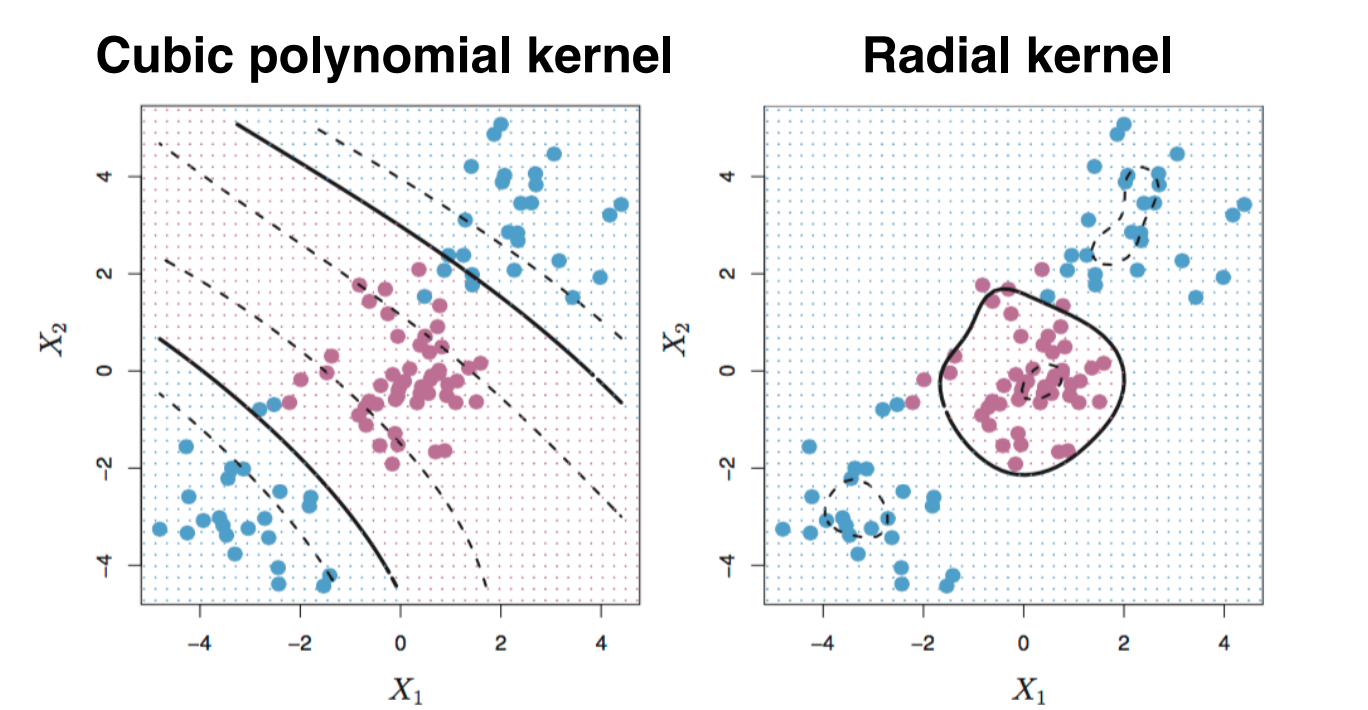
\includegraphics[width=0.9\textwidth]{images/support-vector-machines/support-vector-machines-22.png}
\end{frame}


\begin{frame}{SVM Summary}

\textbf{Pros:}
\begin{itemize}
    \item Regularization parameter $C$ helps avoid overfitting
    \item Use of kernel gives flexibility in shape of decision boundary
    \item Optimization problem is convex — unique solution
\end{itemize}

\textbf{Cons:}
\begin{itemize}
    \item Must tune hyperparameters (e.g. $C$, kernel function)
    \item Must formulate as binary classification
    \item Difficult to interpret
\end{itemize}

\end{frame}


\begin{frame}{SVM with 3+ Classes}

\begin{itemize}
    \item SVMs are designed for binary classification, given the nature of a separating hyperplane.
    \item We can adapt SVMs to perform classification when we have more than 2 classes.
    \item Popular approaches:
    \begin{itemize}
        \item One-versus-one
        \item One-versus-all
    \end{itemize}
\end{itemize}

\end{frame}


\begin{frame}{One-versus-one Classification}

\begin{itemize}
    \item Construct an SVM for each pair of classes.
    \item For $k$ classes, this requires training $k(k-1)/2$ SVMs.
    \item To classify a new observation:
    \begin{itemize}
        \item Apply all $k(k-1)/2$ SVMs to the observation.
        \item Take the most frequent class among the pairwise results as the predicted class.
    \end{itemize}
    \item \textbf{Con:} computationally expensive for large $k$.
\end{itemize}

\end{frame}


\begin{frame}{One-versus-all Classification}

\begin{itemize}
    \item Construct an SVM for each class against the $k-1$ other classes pooled together.
    \item For $k$ classes, this requires training $k$ SVMs.
    \item Distance to separating hyperplane is a proxy for classification confidence.
    \item To classify a new observation:
    \begin{itemize}
        \item Choose the class with the highest confidence (i.e., farthest from the hyperplane).
    \end{itemize}
    \item \textbf{Con:} may exacerbate class imbalances; distance to hyperplane may not correspond well to confidence.
\end{itemize}

\end{frame}
